\documentclass[a4paper, 12pt]{article}

%\usepackage[portuges]{babel}  for portuguese translate some Contents
\usepackage[utf8]{inputenc}
\usepackage{amsmath}
\usepackage{indentfirst}
\usepackage{graphicx}
\usepackage[colorinlistoftodos]{todonotes}

\begin{document}

\begin{titlepage}
	\begin{center}

\vspace{10pt}
\begin{figure}[!ht]
\centering

\includegraphics[scale=0.2]{img/logo_university.png}
\end{figure}


\huge{Universidade Federal de Pernambuco}
\huge{Centro de Informática}

        
        \vspace{85pt}
        
		\textbf{\LARGE{Machine Learning for Hand Gesture Recognition Applied to LIBRAS (Brazilian Sign Language)}}\\
		\vspace{35pt}
		\large{Discipline: Introduction to Computing - IF668[X]}
		\vspace{80pt}
		
	\end{center}
	
	\begin{flushleft}
		\begin{tabbing}
			Students\qquad\qquad\= Eric Vinícius de Lima[X]\\
			\>Michel Leonidas Aleixo da Silva[X]\\
			Professor\> Adriano Lorena Inacio de Oliveira[X] \\
			Time\> Tuesday - 10:00-12:00 AM\\
		
	\end{tabbing}
		  
	\end{flushleft}
	
	\begin{center}
		\vspace{25pt}
		Recife, October 24, 2021
	\end{center}
\end{titlepage}



%  [https://www.cin.ufpe.br/~if668/#]
%  [https://www.cin.ufpe.br/~evl/]
%  [Michel Web Site link, men]
%  [http://lattes.cnpq.br/5194381227316437]

%%%%%%%%%%%%%%%%%%%%%%%%%%%%%%%%%%%%%%%%%%%%%%%%%%%%%%%%%%%
\newpage
\tableofcontents
\thispagestyle{empty}

\newpage
\pagenumbering{arabic}

%%%%%%%%%%%%%%%%%%%%%%%%%%%%%%%%%%%%%%%%%%%%%%%%%%%%%%%%%
%%%%%%%%%%%%%%%%%%%%%%%%%%%%%%%%%%%%%%%%%%%%%%%%%%%%
\section{Introduction}

After an introductory class on Machine Learning given by Professor Adriano L. I. Oliveira [X], a project was requested with the general objective of applying this knowledge of Artificial Intelligence in practice. Building a program that involved machine learning with models based on Text, Images, Numbers or Sounds, applicable to any real or non-real situation.

The Brazilian Sign Language - LIBRAS - is considered official in the country since 2005 [X], but even with more than 10 million hearing impaired people [X], it is still not taught in public schools, making this language learning even more difficult and, consequently, the communication with a hearing impaired.

With that, we decided to develop an application that uses Machine Learning capable of judging with precision if the gesture made with the hand is or not a vowel of the Brazilian Sign Language, through a webcam.

\begin{figure}[!ht]
\centering
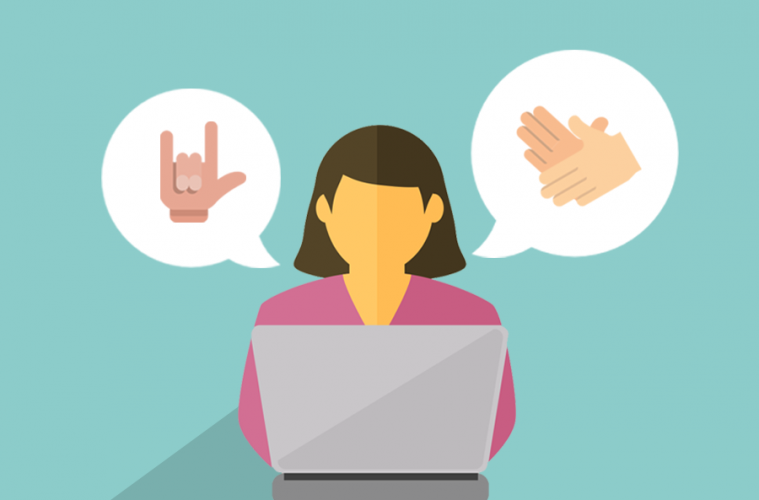
\includegraphics[scale=0.2]{img/inclusion.png}
\caption{Inclusion and accessibility of hearing impaired [X]}
\label{figure_1}
\end{figure}

%  [http://lattes.cnpq.br/5194381227316437]
%  [http://www.planalto.gov.br/ccivil_03/_ato2004-2006/2005/decreto/d5626.htm]
%  [https://www.ibge.gov.br/apps/snig/v1/?loc=0&cat=-1,-2,-3,128&ind=4643]

%  Image: http://www.dfe.uem.br/comunicauem/2018/10/03/inclusao-e-acessibilidade-dos-deficientes-auditivos/




%%%%%%%%%%%%%%%%%%%%%%%%%%%%%%%%%%%%%%%%%%%%%%%%%%%%%%%%%%%%%%%
\section{Tools Used}

For this experiment, the programming language Python [X] was used together with the Mediapipe[X] and OpenCV[X] frameworks, in addition to the Machine Learning for Kids [X] platform for processing the results with the Watson Assistant from IBM[X].

\begin{figure}[!ht]
\centering
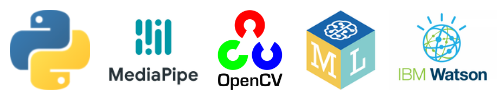
\includegraphics[scale=0.9]{img/tools.png}
\caption{Tools used in this project}
\label{figure_2}
\end{figure}


%  https://www.python.org/
%  https://mediapipe.dev/
%  https://opencv.org/
%  https://machinelearningforkids.co.uk/
%  https://www.ibm.com/watson



%%%%%%%%%%%%%%%%%%%%%%%%%%%%%%%%%%%%%%%%%%%%%%%%%%%%%%%%%%%%%%

\section{Experimental Procedure}

Initially, it was studied how the recognition of a hand by the computer works. We can usually represent it computationally as a 21-vertex graph. To reduce complexity, we decided to work with just 11 of them.
 
\begin{figure}[!ht]
\centering
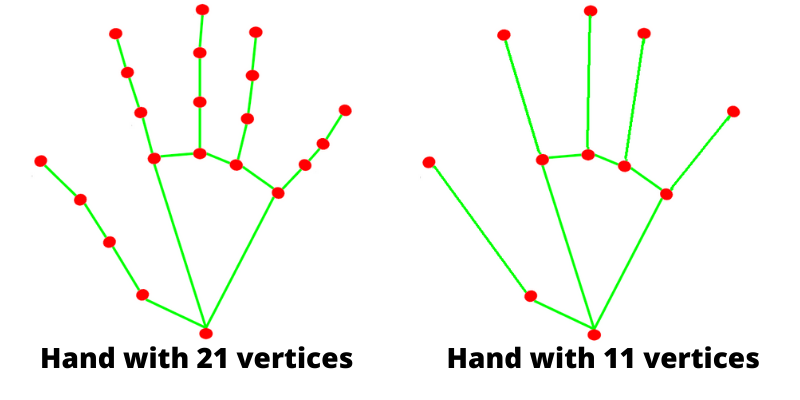
\includegraphics[scale=0.4]{img/hand_vertices.png}
\caption{Hand with different amount of vertices}
\label{figure_3}
\end{figure}

Also, it was decided to judge only the vowels and not the entire alphabet in LIBRAS. Machine Learning for Kids allows only 10 labels to work with numbers. Each vertex has a coordinate containing 2 values: x and y axis. An impediment was then introduced, so it was decided to further reduce the number of vertices, now to just 5. The most relevant vertices were then chosen, following the following gestures:
 
 
 \begin{figure}[!ht]
\centering
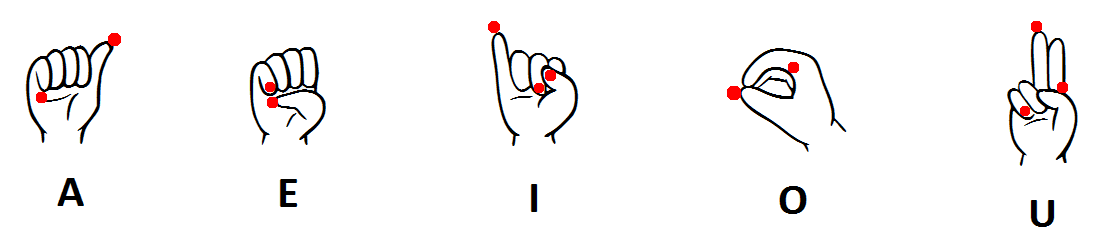
\includegraphics[scale=0.3]{img/hands_gestures.png}
\caption{Vowels in LIBRAS with main vertices}
\label{figure_4}
\end{figure}
 
Following the vertex naming adopted by Mediapipe, the chosen vertices were: 0-wrist, 4-thumb-tip, 5-index-finger-mcp, 12-middle-finger-tip and 20-pinky-tip. With that, the elaboration of the project code was started, and it was divided into 3 parts:






\newpage
\subsection{Data Collect:}
This first part of the project was to use the mentioned libraries to collect the data and treat. The OpenCV was then used to recognize a camera and perform some image settings. Then, we use some solutions present in Mediapipe, to detect and recognize hands, in addition to printing them on the screen. MediaPipe treats the hand with 21 vertices, so we treat these vertices to only take 5 of them and eject the z-axis as it is not needed for the project.

Finally, it was possible to collect, through keys pressed on the keyboard, the x and y axes of each of the chosen vertices.

 \begin{figure}[!ht]
\centering
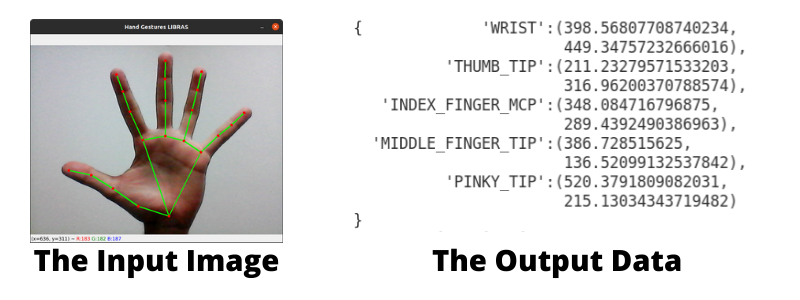
\includegraphics[scale=0.5]{img/data_collect.png}
\caption{Collecting Data}
\label{figure_6}
\end{figure}







\subsection{Populate Training Database:}
To communicate with Machine Learning for Kids, we use its API, in which it is possible to request the classification of data and also request the filling of the training database, and integrate it into the project through the Python Request library [X]. For this, another module responsible for making this communication, was created in addition to generating an API access key directly in Machine Learning for Kids, as well as performing other configurations, such as creating labels for the vowels that will be filled.

 \begin{figure}[!ht]
\centering
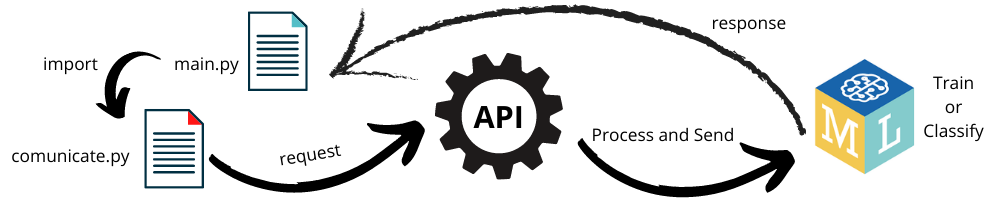
\includegraphics[scale=0.5]{img/api_diagram.png}
\caption{API Diagram}
\label{figure_5}
\end{figure}

%  https://docs.python-requests.org/en/master/




\subsection{Training the IA:}
All computer training is performed by Watson [X], who uses Convolutional Neural Network and linear regression models for classification. Thus, 40 gestures were added for each vowel, made by different people, with right and left hands and on different webcams, to generate greater precision in the results.

%  Show some images for this


%%%%%%%%%%%%%%%%%%%%%%%%%%%%%%%%%%%%%%%%%%%%%%%%%%%%%%%%%%%%
\section{Results Analysis}

After training, some tests were performed for each gesture and the following accuracy results were obtained:

\begin{table}[h!]
    \centering
    \begin{tabular}{ |c|c|c| } 
    \hline
    \multicolumn{3}{|c|}{Results Analysis - 08/22/2021} \\
    \hline
    Gesture & Number of Tests & Accuracy Average \\
    \hline
    A & X & X\% \\ 
    \hline
    E & X & X\% \\
    \hline
    I & X & X\% \\
    \hline
    O & X & X\% \\
    \hline
    U & X & X\% \\
    \hline
    \end{tabular}
    \caption{Results Analysis}
    \label{tab:results_analysis}
\end{table}


%%%%%%%%%%%%%%%%%%%%%%%%%%%%%%%%%%%%%%%%%%%
\section{Conclusion}

...



%%%%%%%%%%%%%%%%%%%%%%%%%%%%%%%%

\section{References}

...

%[1] ...

%[2] ...

\end{document}